\documentclass[a4paper, 12pt]{article}

\usepackage{graphicx}

\begin{document}

	\title{Optimization of time}
		\author{Nick Wang}
		\date{\today}
	\maketitle	

	\tableofcontents

	\part{Interpertation of the problem}
		\section{Introduction}
		\paragraph
		\indent In popular games like Fortnite and PUBG of the battle royale genere, 100 players are dropped off a plane at the beginning of each round. As I played this game more and more, one question has been asked many many times: How to land on the ground in the shortest time possible? At the time I first asked this question, I was fearful of the mathematics involved in such a problem goes beyond my capability, but with knowledge obtained this year and some basic assumptions,  it is possible to approach this problem by disecting it into smaller components.
		\paragraph
		\indent Another angle this problem can be looked at, with some slight modifications, in a more realistic scenario is when a squad of paratroopers is assigned the task to parachute to a given location, what is fastest way possible for the paratroopers to complete this task? 
		\paragraph
		\indent The two approaches to this problem may first seem similar, but they differ slightly. If in a completely realistic environment, meaning a complete replication of what would happen in the real world, the first scenario being a computer simulation would introduce altered physics such as different gravitational acceleration, different air resistance, etc,  whereas in the second scenario theses values would reflect the real data. But from a mathematical point of view, the difference in these variables would meant a different coefficient in some equations, while a general equation can be applied onto both scenarios. Later we will take a close look and investigate the details of each.
		
		\section{The Problem}
		\paragraph
		\indent  The problem told in plain English is as stated: An object, in this case a player, is thrown off an airplane flying in a fixed, predetermined, straight path over a field. The object then proceed to glide in any direction desired while falling downwards towards the ground. Below a certain height is reached, the object then opens up a parachute to slow its descent. The aim is to find the shortest possible time it would take for this object to reach any point on the field.
		\begin{figure}
			\centering
			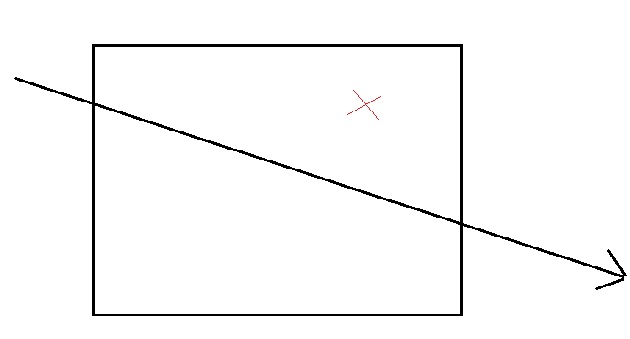
\includegraphics[width=0.5\textwidth]{map.jpg}
			\caption{A map that is representative of such game is shown above, the path the vehicle travels is marked by the dotted lines}
		\end{figure}

		\section{Mathematical reproduction of the problem}
		\paragraph
		\indent To better understand what is being asked, we need to dissect the problem into its components and understand what are the factors that may effect the time that it would take for an object to reach the ground. The first step is to realize that the total time it will take is the sum of the time this object is on the vehicle following a fixed path at a fixed velocity, stage 1, and the time the object is off the vechile and is free to control its movement, stage 2. 	
		\paragraph	
		\indent During stage 1 since the path and velocity are constant, thus the duration of stage is only dependent on the time at which stage 2 begins, or the arbitrary time the object leaves the vechile. Thus if stage 2 starts at $t=a$ and, then the duration of stage 1 is $a$. 
		\paragraph
		\indent Stage 2 consists of 2 sub-stages, first sub-stage  is when the object is first thrown off the vechile and is in a controled freefall, where the angle of falling can be manipulated. During this stage the velocity will be taken as a vector quantity, and the three components, or the composite movement in x,y,and z direction will determine overall velocity. The second sub-stage is when the object reach a certain altitude and opens its parachute, which will slow this object to a constant speed, and its velocity will be evaluated similiarly to the first sub-stage as a vector. The duration of both stages will mostly be determined by the angle of approach, which changes the horizontal distance traveled through out the entire stage. 

		\section{Assumptions and definitions}
		\paragraph
		\indent The combination of the two stages produce a simplified mathematical representation of the problem. But with further thought we would realize that this representation avoided consideration of factors such as air resistance and terminal velocity. Such factors, as mentioned in the introduction, need to be considered differently in the two different scenarios presented.
		\paragraph 
		\indent In the scenario of a computer simulated environment, such values are completly arbiturary to the designer's will. Since this work will not be specific to a single instance of such computer games, a general observation will be made. Thus in this calculation we will redefine the following for the purpose of simplification:
		\begin{enumerate}
			\item[-] Air resistance: Air resistance will be ignored.
			\item[-] Initiation: At the instant the object leaves the vehicle, the object assumes 0 velocity and is stationary relative to the ground.
			\item[-] Terminal velocity: The falling object will reach an arbitrarily defined terminal velocity instantly, and keep falling at this velocity in stage 1 until stage 2 is reached.
			\item[-] Deceleration: The instance stage 2 is reached, the object will release a parachut, and will slow down and descend at terminal velocity, while horizontal velocity will not affect on terminal velocity.
			\item[-] Velocity: Velocity will be considered as a sum of components in x,y and z direction as a vector. The magnitude of velocity will remain constant as the terminal velocity.
			\item[-] Vehicle velocity: Vehicle will be travelling at a greater velocity than the terminal velocity of the object.
		\end{enumerate}
		\paragraph
		\indent In the second scenario,more realistic physics will be applied as following:
		\begin{enumerate}
			\item[-] Air resistance: Air resistance will be ignored.
			\item[-] Initiation: At the instant the object leaves the vehicle, the object assumes velocity of the vehicle, and is stationary relative to the vehicle.
			\item[-] Terminal velocity: The falling object will reach an arbitrarily defined terminal velocity shortly after leaving the vehicle by accelerating at $g=9.8m/s^2$, and keep falling at this velocity in stage 1 until stage 2 is reached.
			\item[-] Deceleration: The instance stage 2 is reached, the object will release a parachut, and will slow down the object instantly to its stage 2 terminal velocity.
			\item[-] Velocity: Velocity will be considered as a sum of components in x,y and z direction as a vector. The magnitude of velocity will remain constant as the terminal velocity.
			\item[-] Vehicle velocity: Vehicle velocity is irrelevant in this scenario, since the object assumes the velocity of the vehicle.
		\end{enumerate}
		\paragraph
		\indent By setting up the two scenarios of the same problem in this fashion we have greatly simplify the problem into its essence. Nuances like air resistance will definitively introduce a greater error to the overall calculation, but it is negligible compared to other more important factors. Furthermore the first scenario is a simplified presentation of a real-life scenario, whereas scenario 2 follows physics much more strictly. Solving scenario 1 first would most likely provide some insights into the harder problem.
		this part will explain and examine all the variables involved in the calculation and define the assumptions that will be made in the calculation, such as that air resistence is processed in a non-realistic way, and most models of physics will not represent the real world since the are based on the game engine.

	\part{Speculations, methods, and solutions}
		\section{Speculations}
		\paragraph
		\indent With the problem and variables defined, we will now look at the problem as a whole and provide some speculations. We will now only look at scenario 1 unless otherwise specified. As explained in Part I Mathematical Reproduction of the Problem, the overall time is the duration of stage 1 and 2 combined, and the aim is to minimize this sum. The duration of stage 2 is completely dependet on stage 1. If the object remained on the vehicle travelling on a fixed path, it will retain a greater horizontal velocity until leaves the vehicle. This means the longer the object remains on the vehicle, the faster it will reach the horizontal location of destination. If the object initiates the freefall, its horizontal will be much lower, but it soon gains vertical velocity. This means the sooner the object initiates freefall, the sooner it will reach the desired vertical location, the land. According to these observations, a few general conclusions can be made:
		\begin{enumerate}
			\item[1] The furthest distance the object can reach is a radius around the point where the object leaves the vehicle, and this radius is limited. Thus if the object leaves the vehicle way too early, or from a mathematical prospective, as the beginning time of stage 2 shifts further towards negative infinity, the object will never reach the desired location. Thus we can conclude that one mustn't drop too early.
			\item[2] If the vehicle goes beyond the point on the path that is shortest distance from the destination, the drop path is symmetrical to the path before reaching this point. This means 
			\item[-] Terminal velocity: The falling object will reach an arbitrarily defined terminal velocity shortly after leaving the vehicle by accelerating at $g=9.8m/s^2$, and keep falling at this velocity in stage 1 until stage 2 is reached.
			\item[-] Deceleration: The instance stage 2 is reached, the object will release a parachut, and will slow down the object instantly to its stage 2 terminal velocity.
			\item[-] Velocity: Velocity will be considered as a sum of components in x,y and z direction as a vector. The magnitude of velocity will remain constant as the terminal velocity.
			\item[-] Vehicle velocity: Vehicle velocity is irrelevant in this scenario, since the object assumes the velocity of the vehicle.
		\end{enumerate}
		this part will go into deeper details to explain why some of the assumptions are made, and what their implications and effect will have on the final results
		\section{Methods}
		this part will justify how the problem is simplified into different componets and each component will be a single variable optimization problem, and the movement is considered as a vector of x,y,z components. This part will also examine how everything come together and the accuracy of such method
		\section{Potential Solutions}
		this part will speculate on what the optimum solution is by using only logic and reasoning. It will not provide concrete mathematical proof, but it can provide some insights.

	\part{Calculations}
	this will be where all the calculations are explained in details

	\part{Reflection and Conclusion}
		\section{Reflection}
		this part will examine the problems, inaccuracies and improvements that can be made to provide a better assessment of the problem.
		\section{Conclusion}dont 
		this part will conclude the problem

\end{document}